\documentclass{article}
\usepackage[utf8]{inputenc}
\usepackage{fancyhdr}
\usepackage{lipsum}
\usepackage{graphicx}
\usepackage{ulem}
\usepackage{wrapfig}

\title{BROJ $e$ I PRIMENA U FINANSIJAMA\\\large{Seminarski rad u okviru kursa}\\\large{Tehničko i naučno pisanje}\\ \large{Matematički fakultet}}

\author{}
\begin{document}

\maketitle

\begin{center}
    

\section*{\large{ANASTASIJA DIVJAK}}

\paragraph{\normalfont{Student 1.godine Matematičkog fakulteta Univerziteta u Beogradu, smer Informatika}}

\section*{\large{NIKOLINA MILENKOVIĆ}}

\paragraph{\normalfont Student 1.godine Matematičkog fakulteta Univerziteta u Beogradu, smer Informatika}

\section*{\large{KRISTINA MILENKOVIĆ}}

\paragraph{\normalfont Student 1.godine Matematičkog fakulteta Univerziteta u Beogradu, smer Informatika}

\section*{\large{NIKOLA JOVANOVIĆ}}


\paragraph{\normalfont {Student 1.godine Matematičkog fakulteta Univerziteta u Beogradu, smer Informatika}}



\paragraph{\\}
\end{center}
\paragraph{\textbf{REZIME: }\normalfont { Kada je otkriven 1618. godine, broju $e$ nije pridavan veliki značaj. Njegovu pravu ulogu otkriva znatno kasnije švajcarski matematičar Leonard Ojler. Ova konstanta iznosi $e$  2,71828... i predstavlja osnovu prirodnog logaritma. Veliku primenu ima i van matematike, a jedna od njegovih najbitnijih primena je u finansijama. Smatra se da je kao prvobitni problem broja $e$ upravo bio problem vezan za finansije. }}
\paragraph{\normalfont{\textbf{KLJUČNE REČI}: broj $e$, prirodan logaritam, finansije, Leonard Ojler}}




\newpage{}

\title{\Large\centering{{SADRŽAJ}}}

\section{\LARGE Rezultati istraživanja i diskusija}
    \subsection{\Large\normalfont Istorija broja $e$ \hspace{8.1cm} 3}
    \subsection{\Large\normalfont O Leonardu Ojleru \hspace{7.2cm} 3}
    \subsection{\Large\normalfont Osobina broja $e$ \hspace{7.88cm} 4}
    \subsection{\Large\normalfont Ojlerov identitet \hspace{7.7cm} 6}
    \subsection{\Large\normalfont Ojlerova kružnica \hspace{7.5cm} 7}
    \subsection{\Large\normalfont Primena broja $e$ u finansijama \hspace{4.85cm} 8}
    \subsection{\Large\normalfont O Bernuliju \hspace{8.7cm} 8}
    \subsection{\Large\normalfont Značaj u finansijama \hspace{6.75cm} 8}
    \subsection{\Large\normalfont Reference \hspace{9.1cm} 9} 



\newpage{}
\pagestyle{fancy}
\fancyhead{}
\fancyhead[RO,LE]{\textbf{Broj $e$ i primene u finansijama}}

\title{\Large\centering{{REZULTAT ISTRAŽIVANJA I DISKUSIJA}}}

\section*{\uline{Istorija broja $e$}}
\paragraph{\normalfont{Broj e se prvi put pojavljuje 1618.godine u logaritamskim tablicama tj. nakon Neperovog otkrića integrala. Tada mu nije pridavan veliki znacaj i njegovu ulogu u matematici i drugim oblastima otkriva znatno kasnije švajcarski matematičar i fizičar Leonard Ojler}}

\paragraph{\normalfont{Naime, u 17.veku švajcarski matematičar Danijel Bernuli ispitivao je kamatnu stopu i različite dohotke na osnovu učestalosti ulaganja. Ono što je zaključio, a što se sad smatra originalnim problemom broja $e$, jeste da se dobija bolji rezultat ako se češće ulaže novac 
i uzima kamata.}}

\paragraph{\normalfont{Pedesetak godina nakon ovoga, Ojler je napokon izračunao vrednost broja $e$ s obzirom da je Bernuli znao samo da se taj broj nalazi izmedju 2 i 3. Osim što ga je izračunao on je pronašao i formulu kojom je dokazao da je ovaj broj iracionalan.\\}}


\begin{wrapfigure}{r}{0.5\textwidth}
  \begin{center}
    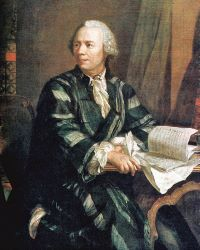
\includegraphics[width=0.48\textwidth]{lojlermodified.jpg}
  \end{center}
  \caption{Leonardo Ojler}
\end{wrapfigure}

\section*{\uline{O Leonardu Ojleru}}

Leonard Ojler rodjen je u Bazelu 15.aprila 1707.godine.
Bio je jedan od najznačajnijih matematičara 18.veka.
Najviše je doprineo u matematičkoj notaciji jer je prvi počeo
da koristi $f(x)$ za zapis funkcije, moderan zapis trigonometrijskih funkcija,$e$ ,$\Sigma$
za sumu,$i$ kao imaginarnu jedinicu.
Pokazao je da se najkraće rastojanje izmedju dve tačke na zakrivljenoj površi pretvara u duž ukoliko se ta površ projektuje na ravan.
Medju manje poznatim Ojlerovim doprinosima nalazi se pokušaj formulisanja teorije muzike u potpunosti zasnovan na matematičkim idejama, koji je napravio napisavši 1739. godine Tentamen novae theoriae musicae,a zatim i brojna druga dela.

\end{document}
